\documentclass{article}
\usepackage[utf8]{inputenc}
\usepackage[a4paper,top=2cm,bottom=2cm,left=3cm,right=3cm,marginparwidth=1.75cm]{geometry}
\usepackage{amsmath}
\usepackage{graphicx}
\usepackage[colorlinks=true, allcolors=blue]{hyperref}

\begin{document}

\begin{titlepage}

\center % Center everything on the page

\newcommand{\HRule}{\rule{\linewidth}{0.4mm}} % Barra horizontal

\begin{figure}[h]
    \centering
    
\includegraphics[width=0.24\linewidth]{images/uniMinho.jpg}
\end{figure}

%\textsc{\Large Universidade do Minho}\\[0.75cm]  % Name of your university/college
\textsc{\Large Licenciatura em Ciências da Computação}\\[0.4cm] % Nome do curso
\textsc{\Large Sistemas de Comunicações e Redes}\\[5cm]

{\Large\bfseries Ensaio Escrito}\\[0.5cm]
%{\huge \bfseries Pesquisa sobre \textit{frameworks} de separação de camadas} % Título
{\LARGE \bfseries   Nível de Ligação Lógica - Ethernet e Protocolo ARP; Redes Sem Fios (IEEE 802.11)} % Título


\vspace{5cm} % Autores
{\bfseries Grupo 28} \\ \vspace{3mm}
Davide Santos (A102938) \\ \vspace{3mm}
Edgar Araújo (A102946) \\ \vspace{3mm}
Pedro Augusto Camargo (A102504) \\ \vspace{3mm}
\vspace{0.2cm}
{Outubro 2023}\\[0.2cm] % Data

\vfill % Fill the rest of the page with whitespace
\end{titlepage}

\tableofcontents
\pagebreak

\section{Parte 1}
\begin{description}
    \item[Analise da fragmentação de pacotes I] 
\end{description}

Foi capturado o tráfego gerado pelo comando: ping -s 6328 marco.uminho.pt

\begin{figure}[h]
    \centering
    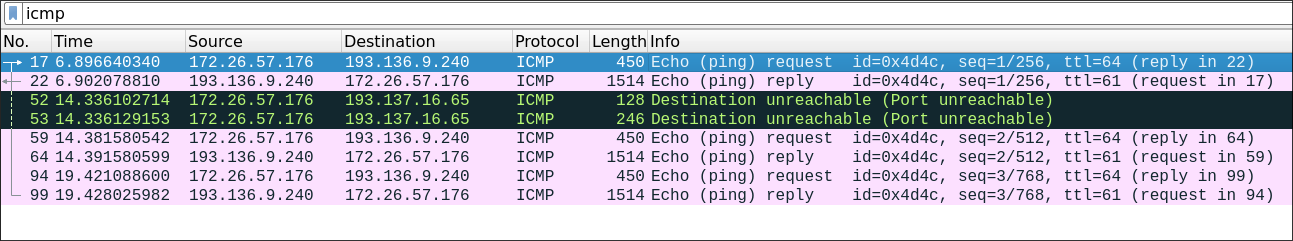
\includegraphics[width=0.8\textwidth]{images/ping.png}
    \caption{\label{fig:ping}Ping}
\end{figure}

\subsection*{a. Localize a primeira mensagem ICMP.}
\subsubsection*{i) Porque é que houve necessidade
de fragmentar o pacote inicial?}
\begin{figure}[h]
    \centering
    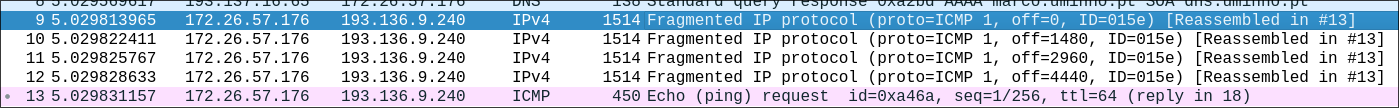
\includegraphics[width=0.8\textwidth]{images/fragment.png}
    \caption{\label{fig:fragment}Fragment}
\end{figure}

A necessidade surge de o facto de o tamanho do pacote ser superior ao MTU da rede, ou seja, não cabe num único pacote. O MTU da rede é de 1500 bytes, e o tamanho do pacote é de 6328 bytes, logo é necessário fragmentar o pacote.

\subsubsection*{ii) Em que equipamento da rede ocorreu
essa fragmentação?}

A fragmentacao ocorreu no computador que enviou o pacote. 

\subsection*{b. Imprima o primeiro fragmento do datagrama IP.}
\subsubsection*{i) Que informação no
cabeçalho indica que o datagrama foi fragmentado?}

A opcao MF, que indica que o pacote foi fragmentado, pode ser observada no wireshark, dentro do campo Flags, no cabeçalho IP.

\begin{figure}[h]
    \centering
    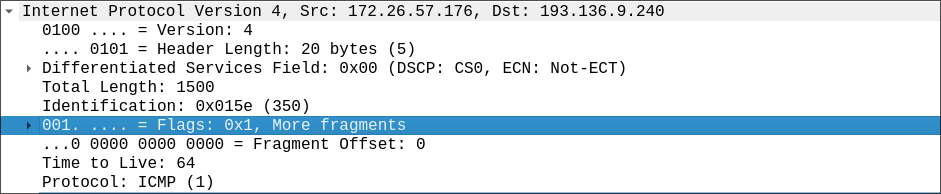
\includegraphics[width=0.8\textwidth]{images/mf.png}
    \caption{\label{fig:more_fragments}More Fragments}
\end{figure}

\subsubsection*{ii) Que informação
no cabeçalho IP indica que se trata do primeiro fragmento?}

O campo Fragment Offset indica que se trata do primeiro fragmento, uma vez que o seu valor é 0.

\subsubsection*{iii) Qual é o tamanho deste fragmento?}

O tamanho do fragmento é de 1500 bytes, tal como indica o campo Total Length.

\subsection*{c. Imprima o segundo fragmento do datagrama IP original. Que informação
do cabeçalho IP indica que não se trata do primeiro fragmento? Há mais
fragmentos? O que nos permite afirmar isso?}

\begin{figure}[h]
    \centering
    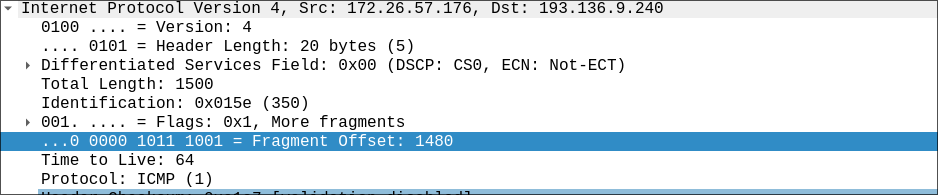
\includegraphics[width=0.8\textwidth]{images/mf_offset.png}
    \caption{\label{fig:more_fragments_offset}More Fragments Com Offset}
\end{figure}

O campo Fragment Offset indica que não se trata do primeiro fragmento, uma vez que o seu valor é 1480. O campo MF indica que há mais fragmentos, uma vez que o seu valor é 1.
Logo basta que: Fragment Offset != 0 $\wedge$ MF == 1 para sabermos que não se trata do primeiro fragmento.

\subsection*{d. Indique os campos que mudam no cabeçalho IP entre os diferentes
fragmentos, e explique a forma como essa informação permite
reconstruir o datagrama original.}

Os campos que mudam sao:
\begin{itemize}
    \item Flag More Fragments (MF)
    \item Fragment Offset
    \item Total Length
\end{itemize}
Os campos que permitem reconstruir o datagrama original, sao o Fragment Offset, e a flag MF, pois estes permitem saber a ordem exata dos fragmentos, de forma a reconstruir tal e qual como antes de ser fragmentado.

\subsection*{e. Como se deteta o último fragmento correspondente ao datagrama
original? Estabeleça um filtro no Wireshark que permita listar o último
fragmento do primeiro datagrama IP segmentado.}

ip.flags.mf == 0

\subsection*{f. Identifique o equipamento onde o datagrama IP original é reconstruído a
partir dos fragmentos. A reconstrução poderia ter ocorrido noutro
equipamento diferente do identificado? Porquê?}

O equipamento onde o datagrama IP original é reconstruído é o servidor de IP: 193.136.9.240, ou seja, o servidor de marco.uminho.pt. A reconstrução poderia ter ocorrido noutro equipamento desde que a MTU fosse superior a MTU da ligacao anterior, ou seja maior que 1500 bytes, e que o equipamento tivesse a capacidade de reconstruir o datagrama original.

\subsection*{g. Por que razão apenas o primeiro fragmento de cada pacote é identificado
como sendo um pacote ICMP?}

Apenas o primeiro fragmento de cada pacote é identificado como sendo um pacote ICMP, pois o conceito de ICMP tem por base os cabecalhos IP, e o conceito de fragmentacao de datagramas IP e relativo ao cabecalho IP.

\subsection*{h. Determine o valor máximo de SIZE sem que ocorra
fragmentação do pacote? Justifique o valor obtido, relacionando-o com o
MTU (Maximum Transmission Unit) da rede.}

Apos observar o output do comando ping no linux:
\begin{figure}[h]
    \centering
    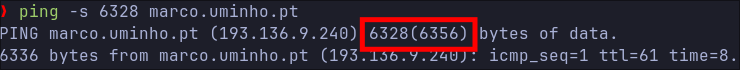
\includegraphics[width=0.8\textwidth]{images/ping_cmd.png}
    \caption{\label{fig:ping_cmd}Comando Ping no Linux}
\end{figure}
Reparei que houve um acrescimo de 28 bytes na informacao enviada, para acomodar todos os cabecalhos essenciais na trasnmissao do pacote.
Logo o valor maximo de SIZE sem que ocorra fragmentacao do pacote e de 1472 bytes, pois 1472 + 28 = 1500 bytes, que e o MTU da rede.

\section{Parte 2}
\subsection{Endereçamento e Encaminhamento IP}
\subsubsection{Atribua um conjunto de endereços IP válidos (públicos) aos diversos sistemas da
GEO, devendo o seu nº de grupo estar presente em pelo menos um octeto da
componente de rede. Use máscaras (prefixos) de rede que respeitem a divisão
clássica de endereçamento por classes (ver a tabela em anexo).}

\subsubsection{Diga, justificando, se na rede está a ser usado encaminhamento estático ou
dinâmico (e.g. baseado no protocolo OSPF - Open Shortest Path First). (Sugestão:
analise os processos que estão a correr em cada sistema (hosts, routers) usando,
por exemplo, o comando ps -ax).}

\begin{figure}[h]
    \centering
    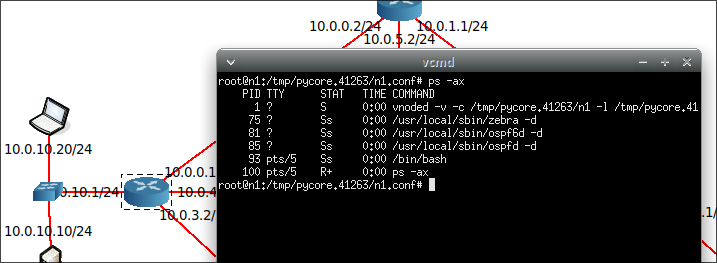
\includegraphics[width=0.8\textwidth]{images/ospf.png}
    \caption{\label{fig:ospf}OSPF no router}
\end{figure}

Conforme a figura acima demonstra, o router esta a usar o protocolo OSPF, logo esta a usar encaminhamento dinamico, pois nao foi necessario especificar as rotas manualmente, e o protocolo ficou responsavel por isso.

\subsubsection{Apague na tabela de encaminhamento do router de cada departamento e do
router central a entrada respeitante à rede da interface wireless do router RISP.
Confirme que os sistemas da GEO deixaram de ter acesso à interface wireless do
router RISP. Usando apenas rotas por defeito, altere as tabelas de
encaminhamento desses routers de forma a tornar novamente acessível o acesso
à Internet através da interface wireless do router RISP.}

Apos apagar a entrada respeitante a rede da interface wireless do router RISP, os sistemas da GEO deixaram de ter acesso a interface wireless do router RISP, pois nao sabem para onde encaminhar os pacotes.
\begin{figure}[h]
    \centering
    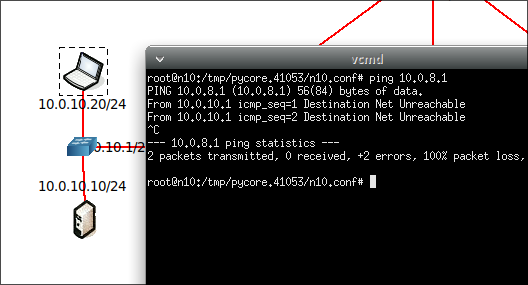
\includegraphics[width=0.8\textwidth]{images/before-route.png}
    \caption{\label{fig:before_route}Antes de routing manual}
\end{figure}

Para retormar o acesso a interface wireless do router RISP, foi necessario adicionar 2 rotas manualmente.
\begin{figure}[h]
    \centering
    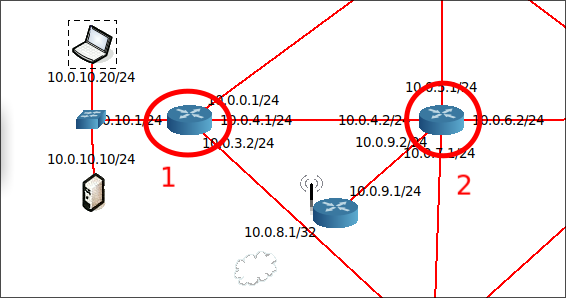
\includegraphics[width=0.8\textwidth]{images/route.png}
    \caption{\label{fig:route}Routing manual}
\end{figure}

\begin{itemize}
    \item No router 1 foi executado o comando: ip route add default via 10.0.4.2
    \item No router 2 foi executado o comando: ip route add default via 10.0.9.1
\end{itemize}

Mas de forma a retornar a conexao de cada departamento a internet, foi necessario adicionar uma rota por defeito no router de cada departamento em direcao ao router central, seguindo o mesmo esquema: ip route add default via "ip do router central".

Apos testar, todos os departamentos conseguiram aceder a internet.

\subsection{Definição de Sub-redes}
\subsubsection{Apresente uma imagem que mostre claramente o esquema de
endereçamento de subredes adotado. Deve justificar as opções tomadas.}

Tem em conta que existem 4 departamentos, apenas seriam necessarios 2 bits para representar as 4 subredes, mas como o enunciado pede que seja reservada pelo menos uma rede para uso futuro, foram reservados 3 bits para representar as subredes, ou seja, 8 subredes.

Logo as subredes seguem o seguinte formato de endereçamento, tendo por base o endereco 10.0.10.xx/24:
\begin{itemize}
    \item Subrede 1 - 10.0.10.0/27 - sendo .0 o valor do ultimo octeto, com o bit \[2^7 = 0 \land 2^6 = 0 \land 2^5 = 0\]
    \item Subrede 2 - 10.0.10.64/27 - sendo .64 o valor do ultimo octeto, com o bit \[2^7 = 0 \land 2^6 = 1 \land 2^5 = 0\]
    \item Subrede 3 - 10.0.10.128/27 - sendo .128 o valor do ultimo octeto, com o bit \[2^7 = 1 \land 2^6 = 0 \land 2^5 = 0\]
    \item Subrede 4 - 10.0.10.192/27 - sendo .192 o valor do ultimo octeto, com o bit \[2^7 = 1 \land 2^6 = 1 \land 2^5 = 0\]
\end{itemize}

\begin{figure}[h]
    \centering
    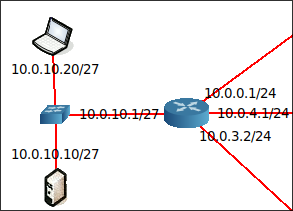
\includegraphics[width=0.8\textwidth]{images/subnetting.png}
    \caption{\label{fig:subnetting}Subnetting}
\end{figure}

\subsubsection{Qual a máscara de rede que usou? Quantos hosts IP
pode interligar no máximo em cada departamento? Quantos endereços
de sub-rede ficam disponíveis para uso futuro? Justifique.}

A mascara de rede usada foi 255.255.255.192, em formato CIDR /27 pois foram reservados 3 bits para representar as subredes, dos ja reservados 24 bits para representar a rede principal.
Sobram-nos 5 bits para representar os hosts, logo temos 32 enderecos disponiveis para hosts, mas como o endereco de rede e o endereco de broadcast nao podem ser usados, ficam disponiveis 30 enderecos para hosts.
A nivel das subredes, ficam disponiveis 4 subredes para uso futuro, pois das 8 subredes possiveis, apenas foram usadas 4.

\subsubsection{Garanta e verifique que a conectividade IP entre os vários
departamentos é mantida. Explique como procedeu.}

Para verificar a conectividade, foi feito ping de cada departamento para cada departamento, e todos os pings foram bem sucedidos.

\end{document}
